\chapter{Physical Environment Monitoring}
\label{chp:pem}

The Physical Environment Monitoring (PEM) system\footnote{PEM originally stood for ``Physics Environment Monitoring" but over time became known as ``Physical Environment Monitoring". The latter definition is used in this dissertation in agreement with contemporary documents.} is a configuration of dedicated sensors at each detector site arranged to observe environmental disturbances. Environmental effects can hinder the sensitivity of an interferometer by increasing the amount of detector noise or by causing an increase in ``glitches" (transient noise artifacts). The first main purpose of the PEM system is to characterize the environmental noise at each site and to help remove any extraneous noise sources (such a loud fan that can be turned off). The second main purpose of the PEM system is to vet detections of GW signals by confirming that environmental sources could not have caused the observed data. This vetting of GW observations is essential to LIGO's ability to claim detections, especially its first.

The main types of environmental disturbances are seismic, acoustic, and electromagnetic, but there are many different types of PEM sensors including: accelerometers, seismometers, microphones, infrasound microphones, magnetometers, thermometers, voltage monitors, radio receivers, tiltmeters, and wind monitors. Different sensors are sometimes used to cover large frequency bands of interest. For example, accelerometers and seismometers look at high and low frequency ground motion respectively. Some of the most important sensor types are outlined in Table~\ref{tab:pem}.

\begin{table*}[t]
\begin{center}
\begin{tabular}{|c|c|c|c|} %{|m{3cm} m{6cm}|}
 \hline
Type & Model & Operating Freq. & Sampling Rate \\ 
 \hline
seismometer & Guralp\textsuperscript{\textregistered} CMG-40T & 0.1\,-\,20 Hz & 256 Hz \\ 
 \hline
accelerometer & Endevco\textsuperscript{\textregistered} 7754-1000 & 1\,-\,900 Hz & 2048 Hz \\
 \hline
microphone & Br\"uel\&Kjaer\textsuperscript{\textregistered} 4130 & 10\,-\,900 Hz & 2048 Hz \\
 \hline
infrasound microphone & Custom & 0.001\,-\,10\,Hz & 256\,Hz \\
 \hline
magnetometer & Bartington\textsuperscript{\textregistered} MAG-03MC & 0\,-\,900 Hz & 2048 Hz \\
 \hline
radio receiver & AOR\textsuperscript{\textregistered} AR5000A & 9 and 45 MHz & 2048 Hz \\
 \hline
 \end{tabular}
\caption{Primary PEM sensors with their sensitive frequency bands.}
\label{tab:pem}
\end{center}
\end{table*}

Environmental noise can couple into the detector's strain channel in a few different ways. The most prominent coupling mechanisms are: changing the length of optical cavities, causing laser beam jitter, modulating the path length of scattered light which then recombines with the main laser beam, and introducing frequency noise~\cite{ana_pem}. In order to characterize and understand how environmental noise affects each detector, PEM ``injections" must be performed at each site. These injections consist of induced noise that is loud enough to be read by PEM sensors and to show up in the detector's strain channel. This allows ``coupling factors" to be calculated, which indicate how significantly different types of noise couple into the detector from different locations. The injected signal is typically a harmonic comb produced by a ramped sawtooth waveform. At each frequency multiple the GW strain amplitude can be divided by the PEM sensor amplitude to calculate a coupling factor. If coupling factors have been measured, then the strain contribution can be estimated for observed environmental noise. For example, if an abnormally large magnetic field was observed at one end station during a GW detection, then the relevant coupling factor could be used to calculate whether that magnetic noise was sufficient to cause the observed GW strain signal. In most situations, the calculated strain contribution is orders of magnitude below what was observed and that noise source can be ruled out as a primary contributor to the GW signal.

The rest of this chapter will summarize the different types of environmental noise, discuss the vetting of GW150914, and look at PEM-related work. A summary of the PEM system and environmental noise during S6 can be found in~\cite{ana_pem}. Robert Schofield's later document outlines the changes for Advanced LIGO~\cite{aLigo_pem}. LIGO's PEM website is also publicly available~\cite{pem_website}.

\section{Environmental Noise}

This section will look at LIGO's main sources of environmental noise and how relevant injections are performed.

\subsection{Seismic and Ground Motion}

Earthquakes, winds, ground traffic, and air traffic are all sources of transient seismic noise. Feedback control systems are used to keep the detector's Fabry-Perot cavities locked on resonance, and seismic motion is the main contributor to the length and angular control signals~\cite{ana_pem}. Large relative motion between in-vacuum mirrors and out of vacuum photodiodes can generate large control signals, which can lead to upconversion and higher frequency noise~\cite{derosa2012global}. The LIGO sites at Hanford and Livingston have different seismic backgrounds due to the different geological structures of their locations~\cite{daw2004long}.

Earthquakes typically produce ground motion in the frequency range of 0.03\,-\,0.1\,Hz, the so-called ``earthquake band". Despite active isolation through the HEPI systems~\cite{matichard2015seismic}, it is common for earthquakes to knock one or more detectors out of lock during science runs. Figure~\ref{fig:EQ_band} shows the passing signal of an earthquake during O1 that knocked LHO out of lock. Storms in the ocean are also sources of seismic noise and produce noise at twice the wave propagation frequency. The resulting noise is within the ``microseism" band of 0.1\,-\,0.3\,Hz~\cite{cessaro1994sources}. Storms in the Pacific Ocean are the primary concern for LHO while storms in the Gulf of Mexico commonly affect LLO. Microseismic noise is always present but can vary by as much as two orders of magnitude over a timescale of days. Due to frequent issues with noise at those frequencies before Advanced LIGO, seismometer signals were used to create a feedforward servo to reduce the coupling of seismic noise into the GW strain data. This reduced microseismic coupling by a factor of 5 during S6~\cite{derosa2012global}. The current Advanced LIGO detectors benefit significantly from active seismic isolation~\cite{matichard2015seismic}.

\begin{figure*}[t]
    \centering
    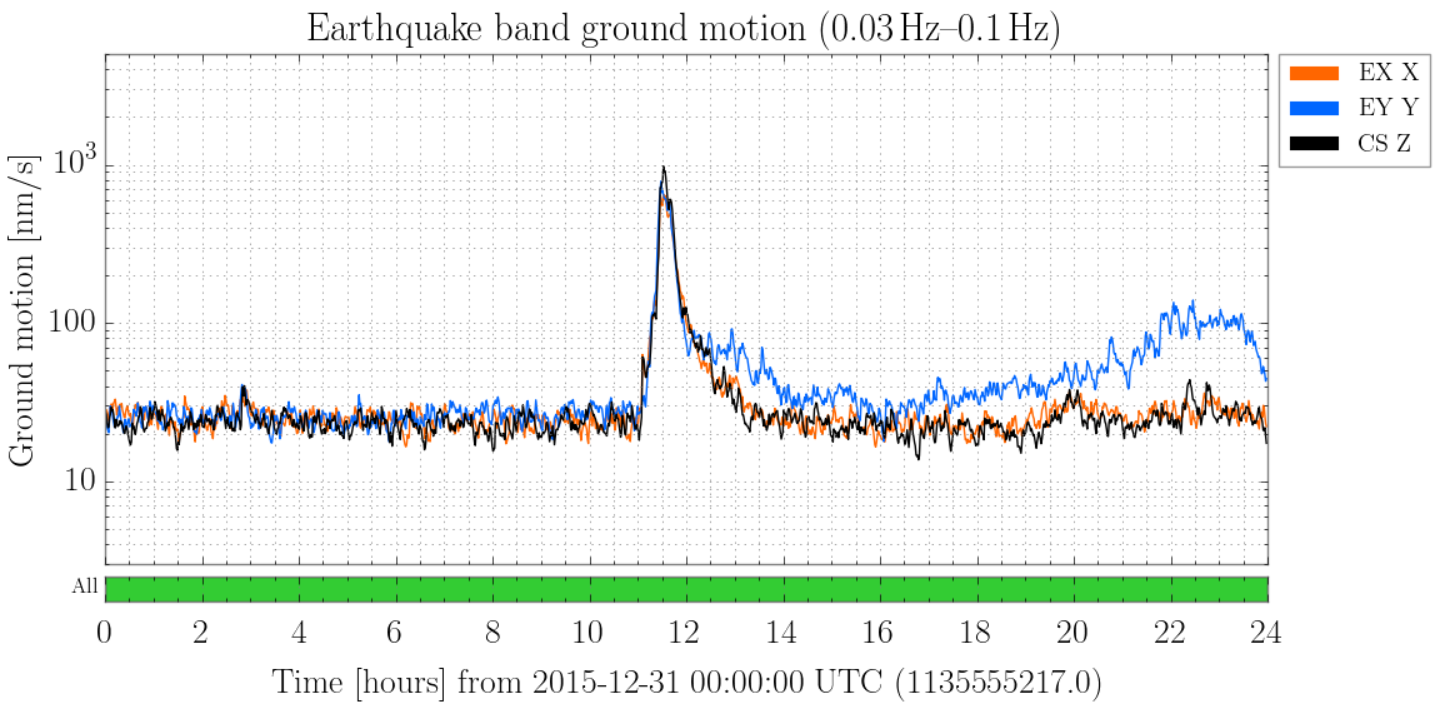
\includegraphics[width=\textwidth]{figures/EQ_band.png}
    \caption{Seismometer data showing a passing earthquake that knocked LHO out of lock during O1. Lock was lost at 11:23:14 UTC.}
    \label{fig:EQ_band}
\end{figure*}

Human activity around the site typically produces motion in the ``anthropogenic band" of 1\,-\,3\,Hz. Naturally this noise varies significantly with the time of day. Winds greater than about 20\,mph can affect the detector's output with most related seismic noise showing up between 0.5\,-\,15\,Hz. Wind can also affect building tilt at low frequencies. Vehicle traffic on nearby highways produces ground motion in the 2\,-\,15\,Hz band. This noise was reduced at LHO by a factor 2 by repaving the main highway next to the site~\cite{ana_pem}. Each site also has its own local noise sources such as pumps, fans, and air conditioning systems. When a local noise source cannot be removed, it is mitigated as much as possible via isolation systems.

Seismic injections are performed with a weighted cart and shaker. The shaker can be moved to different locations and used to inject ground motion at a desired frequency. A different power source is used for the injection equipment with respect to the detector electronics so that current draws won't couple through. In general the injections are performed at an equal distance to the witness sensor and assumed coupling site. 

\subsection{Acoustic}

Known sources of acoustic noise include: electronics fans (above 50\,Hz), chillers (below 60\,Hz), building air control (below 100\,Hz), thermally induced building creeks and thumps (broadband), nearby vehicles (50\,-\,150\,Hz), wind (broadband), and propeller driven aircraft (50\,-\,100\,Hz)~\cite{ana_pem}. Most in-vacuum electronics are well-isolated from sound waves, but several non-vacuum auxiliary systems, such as optical tables, have been found to be significant sources of acoustic coupling. All out of vacuum optical tables have therefore been acoustically insulated with enclosures to minimize the propagation of sound waves.

Acoustic noise couples to the GW strain channel primarily through beam jitter, beam clipping, and beam scattering. Sound waves drive the motion of optical mounts which results in modulations of the primary and auxiliary photodiode signals. Measures have been taken to reduce scattering, such as checking all optical surfaces for stray beams, using beam dumps for all stray light, removing unnecessary protection windows from photodiodes to prevent sensor prompt-reflection backscatter, and using damped material on optical mounts~\cite{ana_pem}.

Acoustic injections are performed with a large 500\,W speaker. This speaker is rolled around to different locations and used to inject loud signals. Acoustic coupling is generally higher in the corner station as opposed to the end stations due to the increased number of optical tables. Figure~\ref{fig:coupling} shows example coupling factors.

\subsection{Electromagnetic}

\begin{figure*}[t]
    \centering
    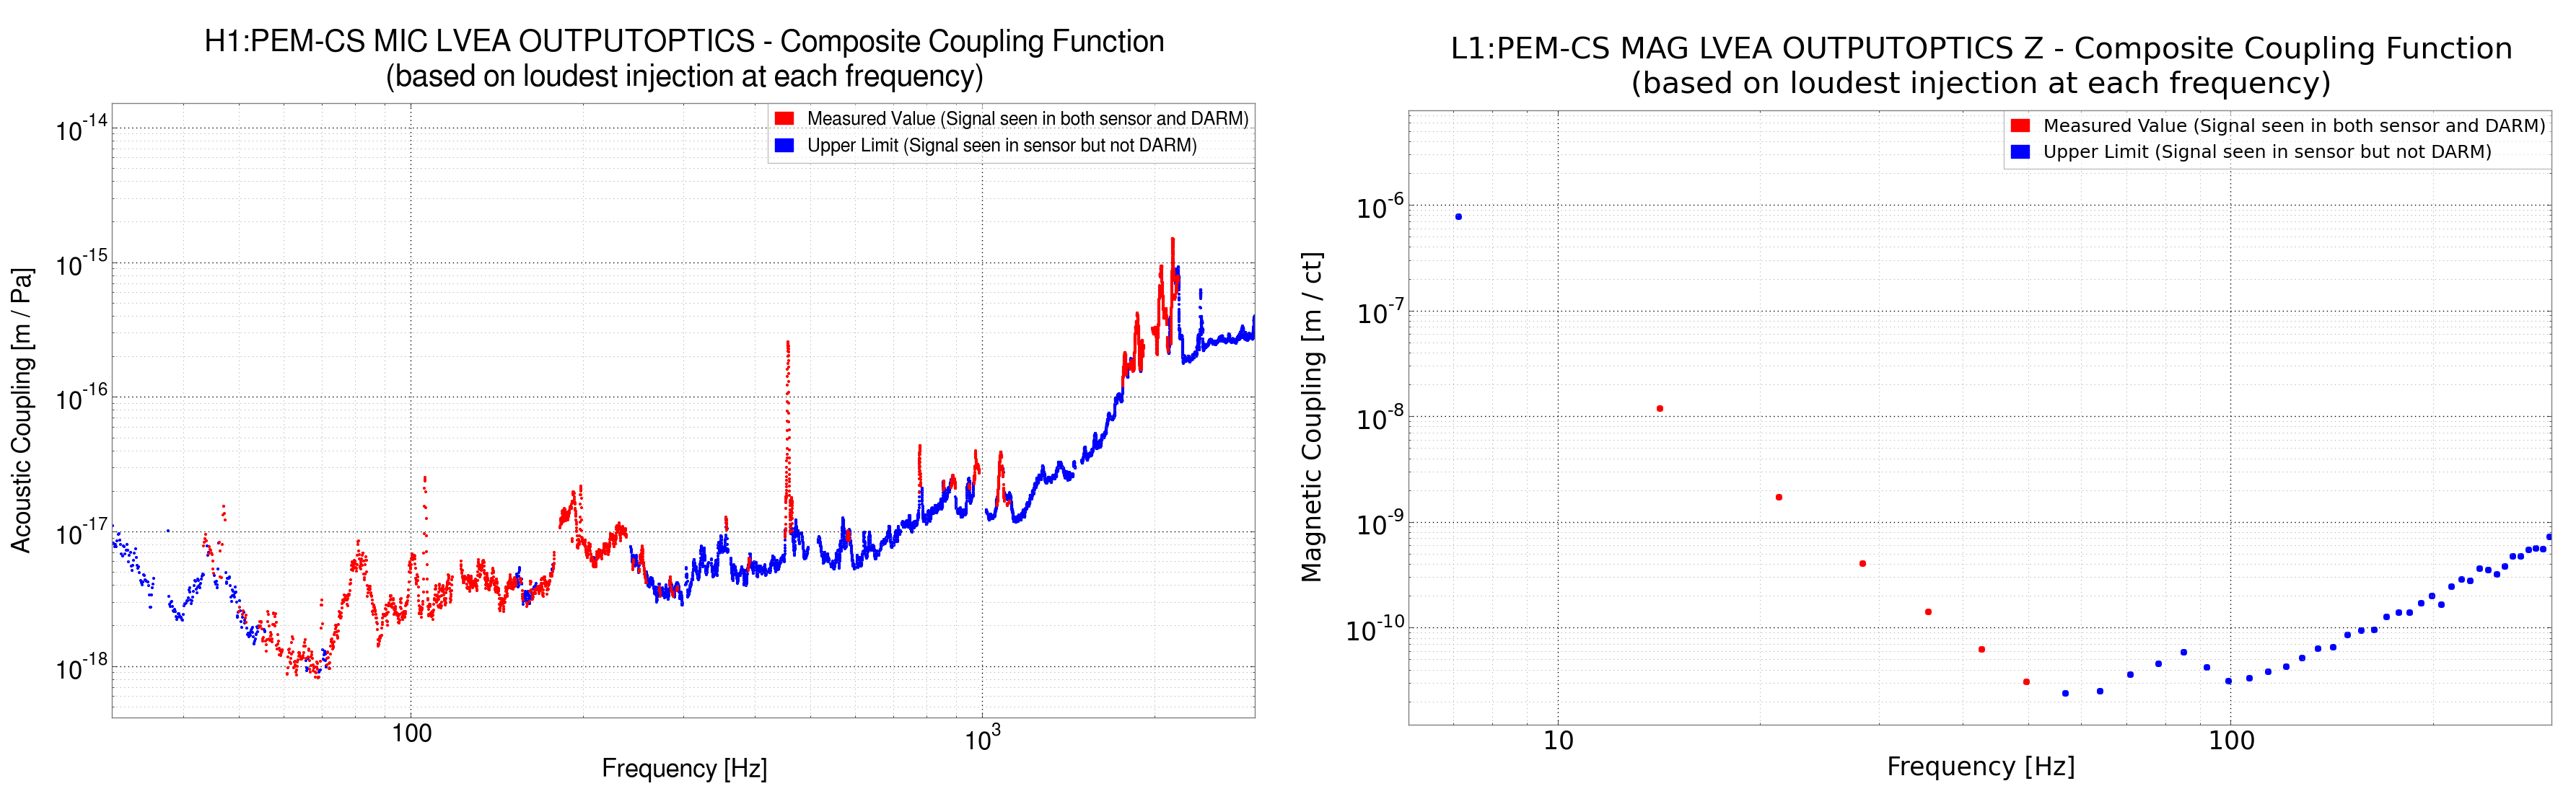
\includegraphics[width=\textwidth]{figures/coupling_factors.png}
    \caption{Left: Coupling factors for a microphone at LHO. Right: Coupling factors for a magnetometer at LLO. Blue data points are upper bound calculations because the injection was not visible in the GW strain channel. Both plots taken from PEM website~\cite{pem_website}.}
    \label{fig:coupling}
\end{figure*}

The LIGO detectors contain a large number of electronics, all of which produce electromagnetic fields. Motors, lights, computers, and building heaters are all examples of potential noise sources. Subtle issues such as flashing lights or significant draws of power can sometimes affect the detector. A refrigerator accidentally left plugged in at a Hanford end station caused mysterious issues for months during O1. PEM magnetometers are located around important electronics to monitor the fields and observe unusual behavior. The GW strain data contains a large 60\,Hz peak due to AC power lines. This peak can hurt LIGO's sensitivity to signals in its vicinity.

Electromagnetic noise couples to the detector primarily through electronic modules, cables, and magnets located on the interferometer optics. Each optic has five magnets, four on its back and one on its side, which are then actuated by coils mounted on the surrounding frame. Uniform magnetic field gradients do not have a direct displacement effect on the optic because the magnets alternate in polarity, however magnetic field gradients comparable to the magnetic field produced by the actuation coil can induce noise in the GW strain channel~\cite{ana_pem}.

Previous versions of the LIGO detectors were hindered by environmental radio frequency (RF) noise. This is because LIGO used a modulation-demodulation scheme (heterodyning) to generate error signals for controlling the length and angular degrees of freedom of the interferometer. Environmental RF noise coupled to the modulation frequencies and produced noise in the strain channel. Before S6, a DC homodyne scheme was adopted to reduce this coupling~\cite{fricke2012dc}. The current Advanced LIGO detectors continue to monitor environmental RF signals at 9 and 45\,MHz, two frequencies of interest for the control systems.

Magnetic injections are performed with a 1\,m (diameter) 100-turn copper coil. This coil is attached to a power source and can be wheeled around the site. The coil is typically located an equal distance from the magnetometer and the coupling site (magnet actuators on the optics). The strain contribution from ambient magnetic fields is usually well below LIGO's noise curve. Example magnetic coupling factors can be seen in Figure~\ref{fig:coupling}. RF injections are performed with an RF source located well outside of the corner station building and are done at the modulation frequencies of LIGO's control systems.

\section{System Installation}

Both LIGO sites underwent large-scale modifications after S6 in preparation for Advanced LIGO. A small number of PEM sensors were able to remain in place throughout the transition but the vast majority had to be removed for hardware upgrades. After the upgrades were complete, the PEM system had to be reinstalled. This installation process was performed over the course of two summers primarily by Robert Schofield, Anamaria Effler, Terra Hardwick, and myself.

Each sensor needs to be located very specifically in order to produce useful, clean data. Microphones are hung away from metallic surfaces to reduce echo and ambient noise. Magnetometers are placed next to specific electronics and must be oriented such that each dimension is properly monitored. Tiltmeters, seismometers, and infrasound microphones are located on the floor outside of vacuum chambers but must be clearly marked and out of the way for site workers. Accelerometers are mostly located in specific locations on the outside of vacuum chambers. They are also attached via epoxy to an insulating surface which is then attached via epoxy to the chamber wall. Other sensors were more difficult to install, such as the accelerometers in the Primary Stabilizing Laser (PSL) room and the RF antennae. The PSL is in a clean room that requires multiple stages of preparation along with specific attire to enter. The accelerometers were then carefully placed on optics tables. The RF antennae had to be installed along the ceiling in the electronics bay and above the corner station vacuum chambers. This required holes to be drilled in the walls while on top of very tall ladders. A two person rope system was then used to run the cable along the ceiling 

All of these sensors and their specific locations are mapped on the PEM website~\cite{pem_website}. As each sensor was installed, its information was put online for future reference along with a photograph of the installed sensor and an example data plot. The example data plots show typical power spectra for ambient noise. The exact location of each sensor was also calculated via trilateration using a laser distance measure and certain precisely measured spots on the floor (used for site construction). These precise coordinates are also on the website and can be theoretically used to calculate the velocity of a propagating wave or the epicenter of an observed disturbance. Figure~\ref{fig:pem_website} shows an example screenshot from the PEM website.

\begin{figure*}[t]
    \centering
    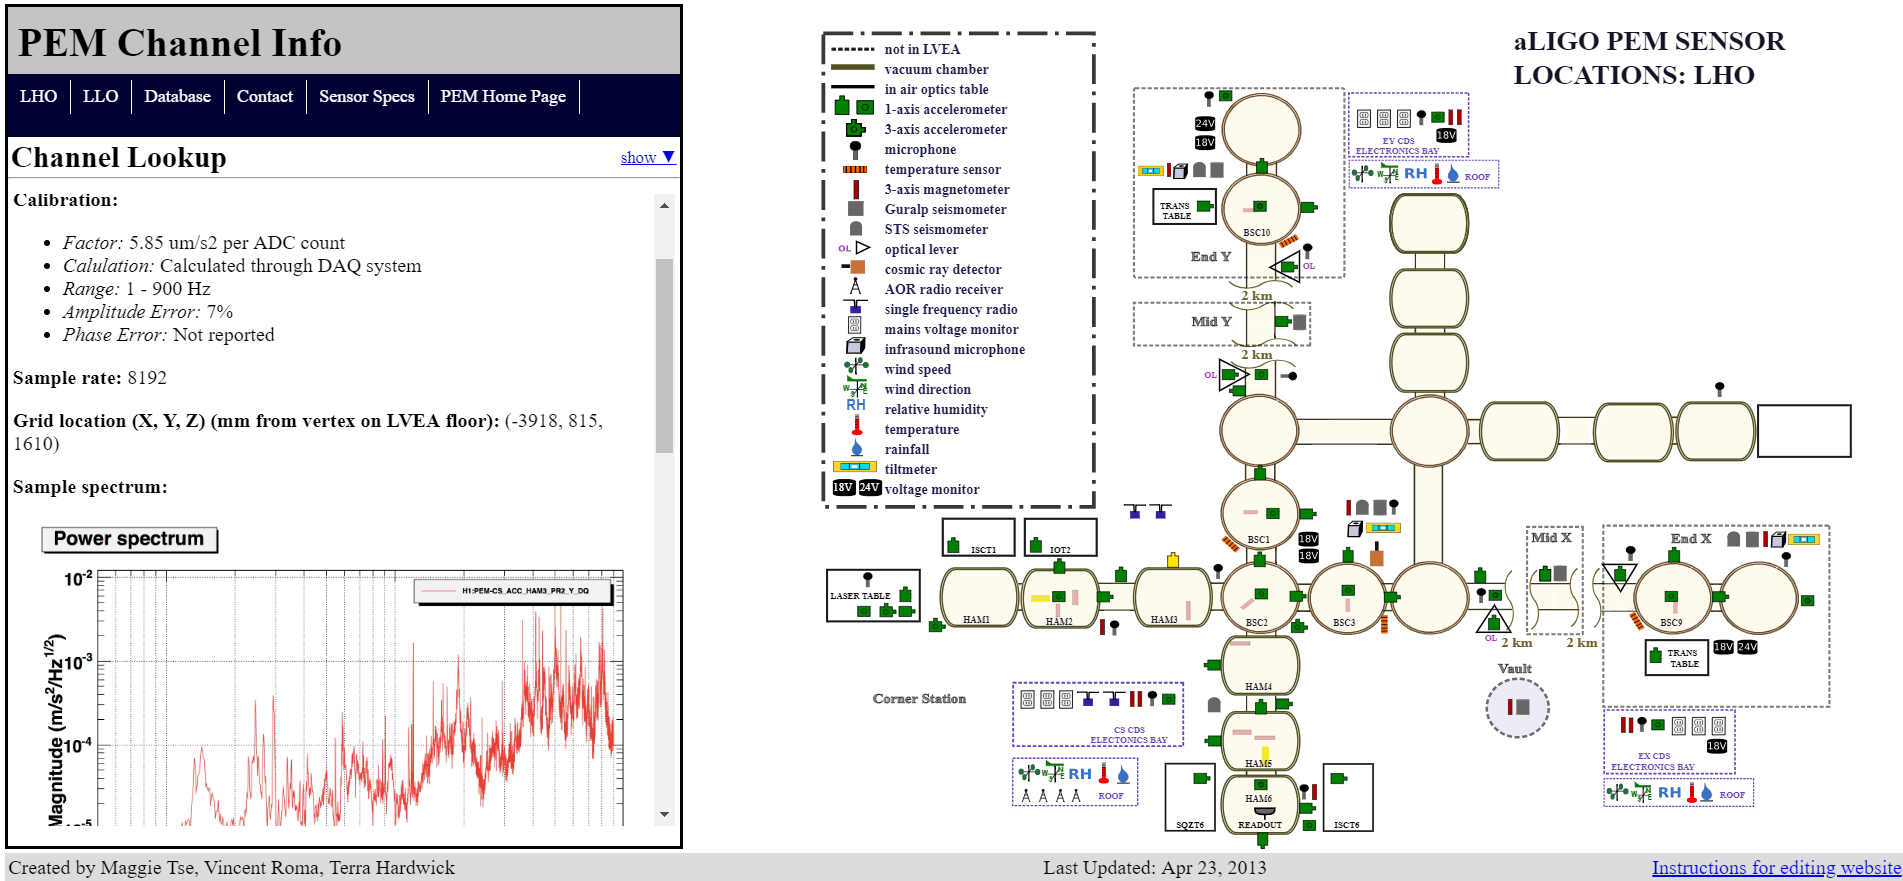
\includegraphics[width=\textwidth]{figures/pem_website.png}
    \caption{Screenshot from the PEM website~\cite{pem_website}. Sensor map on the right is interactive. Clicking on a sensor brings up its hardware information, calibration information, coordinates, example power spectra, and installation photo.}
    \label{fig:pem_website}
\end{figure*}

In addition to installing each sensor, the sensors need to be powered and their data needs to enter LIGO's Data Acquisition System (DAQ). This means that cables had to be ran from the electronics bay out onto the floor. These cables leave the electronics bay and enter the site floor via elevated cable trays above the vacuum chambers. Sometimes these cables must be ran for hundreds of feet, passing along the floor underneath hardware and/or above vacuum chambers 12 feet off the ground. Properly running long cables from the electronics bay to sensors out on the floor requires at least two people and can take hours. After everything is properly installed, the system must be tested. Some sensors simply don't behave properly and must be replaced. The accelerometers are connected to a power supply in the electronics bay which then sends the signal to an Analog-to-Digital Converter (ADC). Some of these older power supplies suffered from significant ``crosstalk", where one accelerometer's signal would cross over into the data of a nearby channel. After extensive testing, these bad channels were avoided and some of the power supplies had to be replaced. All of these cable connections for the PEM system also had to be mapped and documented in the electronics bay. After working with Robert Schofield to install the PEM system at Hanford, Terra Hardwick and I spent the next summer in Livingston installing that PEM system with Anamaria Effler.

The status of PEM sensors is monitored with an algorithm called LigoCAM. LigoCAM was created by Dipongkar Talukder and is accessible from the PEM website~\cite{pem_website}. This algorithm monitors the band-limited root-mean-square (BLRMS) of every PEM sensor to determine when a sensor has come unplugged or has experienced a significant change of state. Students working on site, such as myself, helped to develop and tweak the settings of LigoCAM in order to make it operate as planned. This algorithm continues to run and notifies workers when PEM sensors change state unexpectedly.

\section{Detection Vetting and GW150914}

The LIGO interferometers measure distance more precisely than any device in history. This makes the interferometers incredibly sensitive to environmental effects and hardware glitches. In order to claim an observation of a GW signal, LIGO must be able to guarantee that their signal is extraterrestrial in origin. This was all the more important for the first direct GW observation, GW150914, as previous researchers have incorrectly claimed GW detections in the past~\cite{weber1969evidence}. This section will summarize the PEM detection vetting process with a focus on GW150914. A brief summary of the PEM report is included in the detection paper~\cite{GW150914} and members of the LIGO collaboration can view the full PEM report in the event log~\cite{pem_GW150914}.

The primary concern for a PEM vetting report is whether or not an environmental source could have caused the GW signal. GW150914 was detected at 09:50:45 UTC by both LIGO detectors. At that time, 13-15\% of PEM sensors were inactive or had not yet been fully installed. GW150914 surprised everyone at the tail end of an engineering run, right before the data-taking period was scheduled to begin. Fortunately, sensor redundancy provided good coverage despite the missing channels. Multiple magnetometers were inactive at both sites, but all of those locations had at least one functioning magnetometer. There were plenty of functioning accelerometers and seismometers throughout both sites to ensure that significant ground motion could not go undetected. Every missing channel is listed in the report and its effect on coverage is analyzed. The most important missing channels were the mains voltage monitors at LLO, but voltage glitches also produce magnetic glitches and magnetometers were functioning. In short, both detectors had sufficient coverage to observe environmental influences.

\begin{figure*}[t]
    \centering
    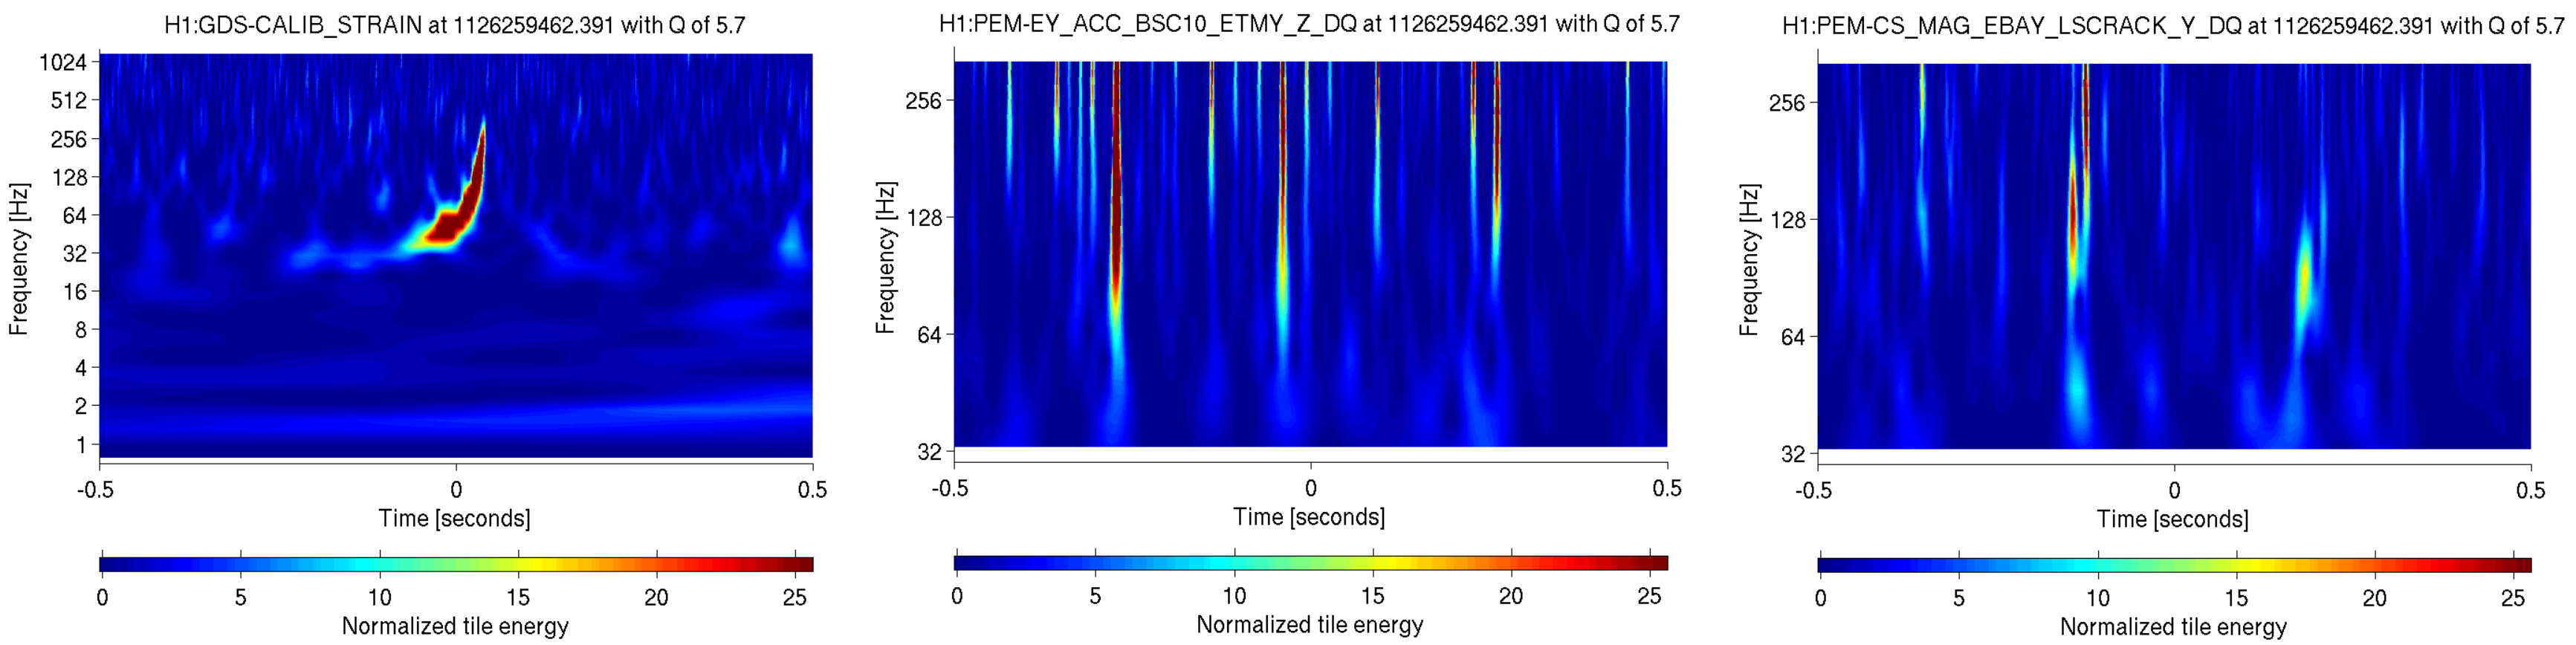
\includegraphics[width=\textwidth]{figures/wdq_plots.png}
    \caption{Omega scan plots from LHO. Left: GW strain channel. Center: Accelerometer on corner station vacuum chamber. Right: Magnetometer in corner station electronics bay. No PEM channels had a time-frequency path similar to the GW signal.}
    \label{fig:wdq_plots}
\end{figure*}

An Omega scan~\cite{chatterji2004multiresolution} is a commonly used spectrogram tool for looking at signals and glitches in LIGO data. Spectrograms are produced for the GW strain channel and any other channels that show increased activity during the event time. Omega scans were ran on every PEM channel for the frequency band 30\,-\,350\,Hz at both sites. This frequency band was chosen because of the time-frequency (TF) path of the signal. Some PEM channels had sufficient noise to produce plots in the Omega scan, but none of them had a TF path similar to the GW observation. Figure~\ref{fig:wdq_plots} shows Omega scan plots of the GW150914 signal and two PEM sensors at LHO. As described earlier in this section, coupling factors can be calculated for PEM sensors that describe how noise sources influence the strain channel. This can be done in terms of amplitude or in terms of SNR. In both cases, the coupling relates the PEM sensor signal to the GW strain signal. SNR coupling factors were used for each PEM sensor in the Omega scan to calculate how loud the signal would have to be to generate the observed strain signal. This was done for all sensors, regardless of TF path. The loudest environmental signal at LHO would have had to have been 31 times louder in order to produce the strain SNR. The loudest environmental signal at LLO would have had to have been 23 times louder~\cite{pem_GW150914}.

In addition to the Omega scans, power spectra were produced for every PEM sensor around the time of the event. Two plots were created, one with 1 second of data, and the other with 64 seconds of data. Spectra for every single PEM channel was plotted against its background levels. Any channels showing unusual noise around the event time were further investigated. No significant concerns were found and Figure~\ref{fig:spectra_plots} shows some example spectra plots for PEM sensors. Spreadsheets with all of the channel information and links to plots were included in the PEM vetting report~\cite{pem_GW150914}. All PEM sensors were checked for abnormal behavior through multiple means, and none showed evidence of an environmental disturbance that could have caused GW150914.

\begin{figure*}[t]
    \centering
    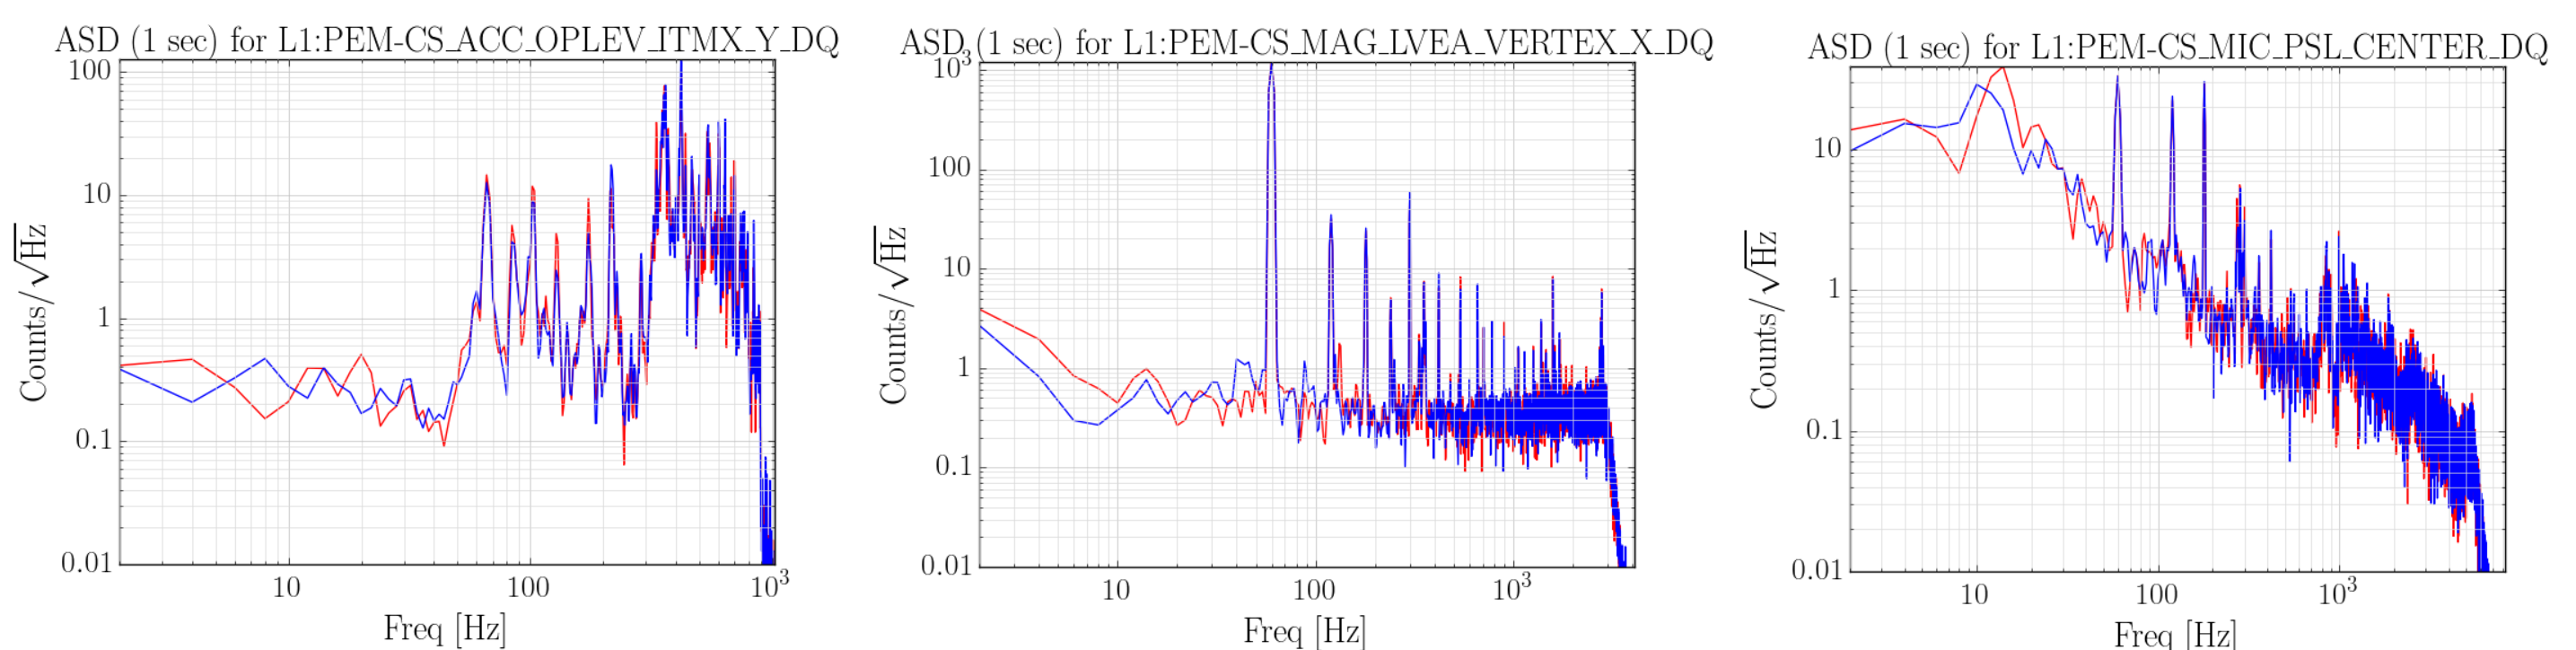
\includegraphics[width=\textwidth]{figures/spectra_plots.png}
    \caption{Spectra plots for three LLO PEM sensors. Left: Accelerometer on optical lever. Center: Magnetometer in corner station. Right: Microphone in PSL room. Plots contain one second of data centered on GW150914 event time. Red trace represents spectra from the event time, blue trace is a reference from 100 seconds before.}
    \label{fig:spectra_plots}
\end{figure*}

It is possible, through upconversion or downconversion, for noise outside of our frequency band of interest to contribute to the observed GW strain signal. One noteworthy mechanism of downconversion is addressed in the PEM report. Non-linear coupling at HAM6 (both sites), produced by intermodulation of the vibration frequency and the OMC length dither (4100 Hz at LHO), can down-convert vibration above 2500\,Hz into the 30-350\,Hz event band~\cite{pem_GW150914}. However, none of the microphones or accelerometers around HAM6 showed any high frequency noise above background levels, indicating that there was no high frequency noise to down-convert. It is also highly unlikely that upconverted or downconverted noise would resemble the transient, chirp-like signal seen in GW150914.

The environment can influence LIGO interferometers through physical contact, electromagnetic waves, static and electric magnetic fields, and possibly high-energy radiation. Environmental influences that propagate near the velocity of gravitational waves and could influence both sites must be monitored. Global-scale high energy radiation events and electromagnetic events are considered, potentially including power grid events~\cite{pem_GW150914}. The Hanford site has a cosmic ray detector located underneath a vacuum chamber. Cosmic rays are unlikely to produce non-random coincidences between detector sites and the cosmic ray environment was quiet around the event time. Certain hardware at both detector sites is synchronized to GPS time, which can produce low-amplitude combs of spectral lines that are coherent between sites. However, there is no reason to expect transient data corruption events that are synchronized between sites. Such events would be also be simultaneous, as opposed to our observed signal which has a reasonable light speed delay between the two detectors. Solar events would be detected by the RF receivers if they were significant enough to affect the strain channel. Solar radio flares would have been blocked (it was night time) and there were no flares around the event time. There were no coronal mass ejection geomagnetic storms. If seismic or acoustic noise happened coincidentally at both sites then it would have been detected by PEM sensors.

The global electromagnetic environment is always examined around a GW event. Generally, any electromagnetic or RF signal that was strong enough to affect the GW strain channel would be detected by the PEM magnetometers, however, data from external electromagnetic and RF observatories is always reviewed. No significant local electromagnetic or RF events were observed around GW150914. Schumann resonances are a lightning driven comb of peaks with the fundamental at about 8\,Hz (given by light travel time around the earth). They do not show up strongly in the event data and there's no reason to believe they would produce the transient GW signal observed. There was a large burst of lightning in Burkina Faso right around the event time that caused some concern, however calculations showed that at that distance it was at least three orders of magnitude too small to create the GW signal. Lightning strikes also release their energy in a broadband fashion, as opposed to the observed chirp. There were many closer lightning strikes that day, none of which affected the detectors.

None of the PEM sensors produced any evidence that an environmental source could have caused GW150914. Data from many external observatories reinforced this conclusion. The PEM vetting process has been streamlined over time as more GW observations have been recorded. Spectra are no longer produced for every PEM channel and the Omega scan process has been greatly improved. The PEM vetting is moving towards full automation, which will be necessary as the LIGO detectors improve their sensitivity. Eventually, GWs from binaries will be observed weekly or daily, requiring a very efficient vetting process.

\section{Noise Correlation Analysis Tool}

During S5 and S6, seismic uponversion was a significant problem for the LIGO detectors. Upconversion refers to low frequency noise that causes higher frequency noise in the strain channel. Upconversion can happen through different mechanisms, sometimes ones that are not obvious. In S5 and S6, microseismic noise (0.1\,-\,0.3\,Hz) caused upconversion due to the Barkhausen effect. The Barkhausen effect refers to suddenly changing magnetic domains in a ferromagnet due to a changing external field. This happened either in the test mass magnets themselves or in the magnetic parts associated with the actuation on the mirrors~\cite{S6_characterization, weiss2008various}. Essentially, something was ferromagnetic that shouldn't have been. These issues lead to the development of software to help find and identify upconversion.

The Noise Correlation Analysis Tool (NCAT) was originally developed by Ryan Quitzow-James. This algorithm compared the band-limited root-mean-square (BLRMS) of a PEM channel to the BLRMS of the GW strain channel in order to find correlated noise bands. The mechanism at play behind this noise correlation is irrelevant. This allowed microseismic noise in seismometers to be correlated to the higher frequency (20\,-\,400\,Hz) strain noise. Each time the code is ran, a set of PEM channels and frequency bands can be chosen. All channels and frequency bands are then searched for correlated noise and a simple web page is produced to display the results. I took over this code and project as my first foray into coding and LIGO-related science. The code was rewritten entirely in Python (previously the BLRMS calculations used a C executable) for simplicity and also to incorporate GWpy, a library of GW-related Python functions. From that point, the math and figure of merit calculations continued to be expanded upon.

NCAT was designed to be ran on large spans of data, sometimes months. The data, for both PEM sensors and GW strain, is then broken up into variable sized sections (usually 16 or 32 seconds long). A one-sided power spectral density (PSD) is calculated for these sections of data which is then used to calculate the BLRMS in the usual way,
\begin{equation}
\label{equ:blrms}
    \text{BLRMS} = \sqrt{\sum_{f=f_{1}}^{f_{2}} \text{PSD}(f) df}
\end{equation}
where $f_{2}$ and $f_{1}$ represent the upper and lower frequency bounds respectively. The formula has been written as a sum instead of an integral because the data is discrete. Once all of the BLRMS calculations have been performed, the data can be plotted and figures of merit can be calculated.

\begin{figure*}[b!]
    \centering
    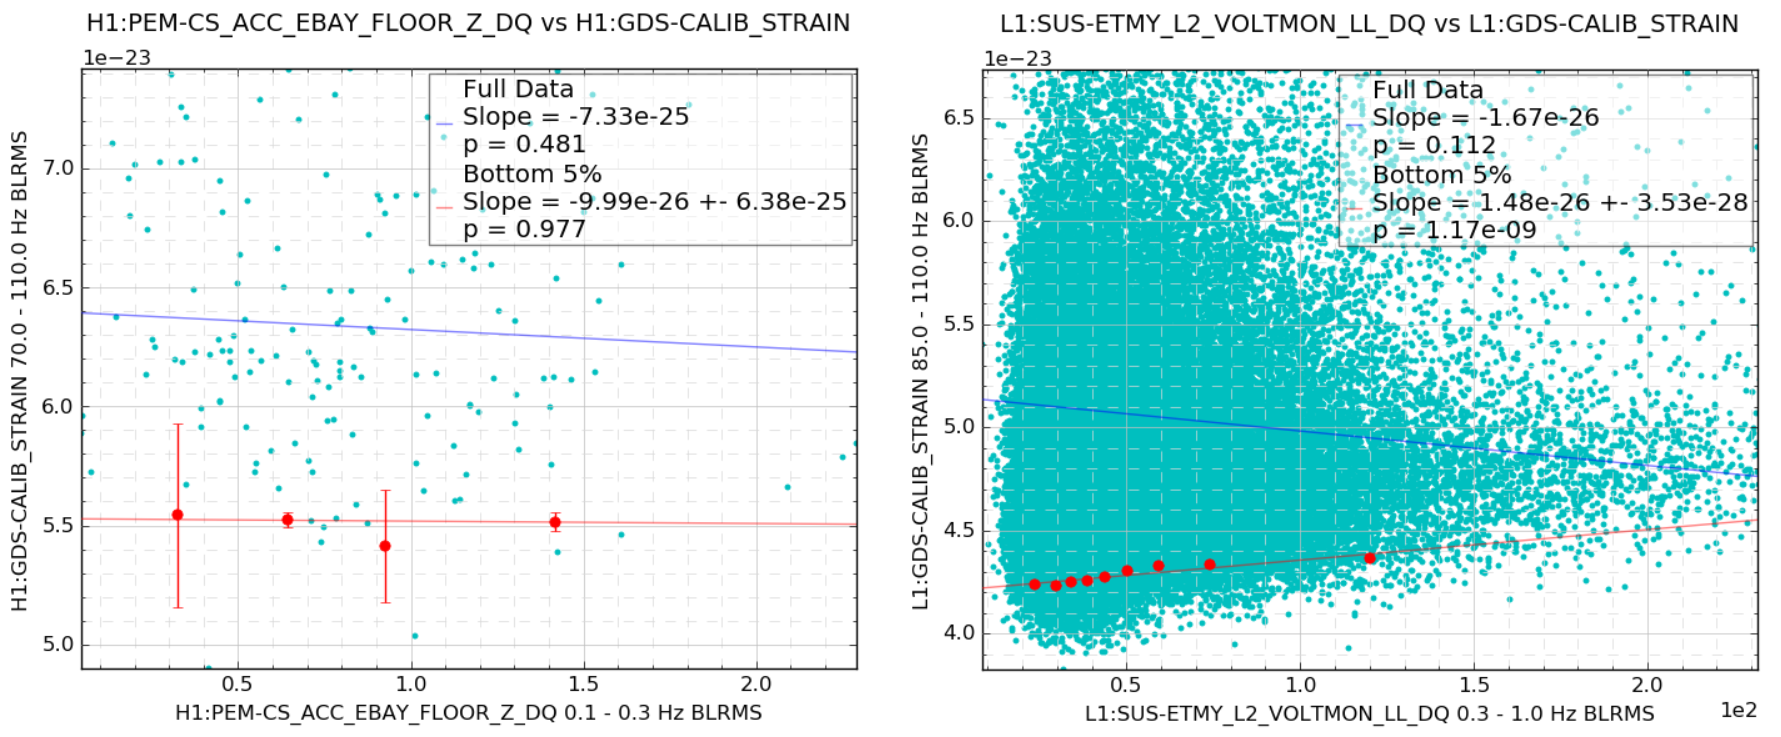
\includegraphics[width=\textwidth]{figures/ncat_plots.png}
    \caption{Example NCAT plots showing low frequency BLRMS for PEM sensors vs higher frequency BLRMS for strain. Left plot shows no evidence of correlated noise with a p-value of 0.977 (bottom 5\%). Right plot shows strong evidence with a p-value of $1.17\times10^{-9}$.}
    \label{fig:ncat_plots}
\end{figure*}

Figure~\ref{fig:ncat_plots} shows two example NCAT plots with BLRMS data. The PEM sensor data is plotted along the x-axis and the GW strain data is plotted along the y-axis. The code is searching for a correlation between these two frequency bands, but the GW strain channel has many noise sources all contributing to its overall signal. For that reason, the quietest strain data points are more useful as they will give a more accurate relationship between the two frequency bands, less corrupted by other noise sources. All of the blue data points are binned horizontally to create the red data points. The binning function is flexible and ensures that each bin has sufficient data points. This is visible in the right plot as the rightmost bin (red data point) is located a significant distance from its nearest neighbor. This is due to the smaller number of data points in this region. The red data points represent the mean of the bottom 5\% (optional) of each bin. When there are sufficient data points the bottom 1\% can be used. Each red data point has error bars based on the standard deviation of the data points used in its calculation. A linear best fit line is then calculated for the red data points. If this line has a significant positive slope, then the two noise bands are correlated. The significance of the slope is determined with a t-test, which results in a p-value for our figure of merit. These statistics are visible in the legend of each plot, for the full data (blue) and bottom 5\% (red).

The linear fit line is calculated using standard formulas, but weights each data point by the inverse square of its standard error (error bars). Data points with large errors will affect the linear fit less significantly. All formulas can be found in numerous statistics textbooks~\cite{freedman2007statistics, stats_shao}. For a series of data points with x and y values, the y-intercept is,
\begin{equation}
\label{equ:y_intercept}
    \text{y-intercept} = \frac{\big(\sum \frac{x_{i}}{e_{i}^{2}}\big) \big(\sum \frac{x_{i}y_{i}}{e_{i}^{2}}\big)-\big(\sum \frac{y_{i}}{e_{i}^{2}}\big) \big(\sum \frac{x_{i}^{2}}{e_{i}^{2}}\big)}{\big(\sum \frac{x_{i}}{e_{i}^{2}}\big)^{2} - \big(\sum \frac{x_{i}^{2}}{e_{i}^{2}}\big) \big(\sum \frac{1}{e_{i}^{2}}\big)}
\end{equation}
where $e_{i}$ represents the standard error  of each data point (error bars in plot). The slope is found similarly as,
\begin{equation}
\label{equ:slope}
    \text{slope} = \frac{\big(\sum \frac{x_{i}}{e_{i}^{2}}\big) \big(\sum \frac{y_{i}}{e_{i}^{2}}\big)-\big(\sum \frac{x_{i}y_{i}}{e_{i}^{2}}\big) \big(\sum \frac{1}{e_{i}^{2}}\big)}{\big(\sum \frac{x_{i}}{e_{i}^{2}}\big)^{2} - \big(\sum \frac{x_{i}^{2}}{e_{i}^{2}}\big) \big(\sum \frac{1}{e_{i}^{2}}\big)}
\end{equation}
with the standard error of the slope (SE) given by,
\begin{equation}
\label{equ:slope_error}
    \text{SE} = \sqrt{\frac{\sum \frac{1}{e_{i}^{2}}}{\big(\sum \frac{x_{i}^{2}}{e_{i}^{2}}\big) \big(\sum \frac{1}{e_{i}^{2}}\big)-\big(\sum \frac{x_{i}}{e_{i}^{2}}\big)^{2}}}
\end{equation}
This standard error of the slope is used directly in our t-test, where our t statistic is defined as~\cite{freedman2007statistics},
\begin{equation}
\label{equ:t_test}
    \text{t} = \frac{\text{slope}}{\text{SE}}
\end{equation}
This value can be converted to a p-value using the cumulative distribution function~(cdf) for a Student's t distribution. Explicitly,
\begin{equation}
\label{equ:p_value}
    \text{p-value} = 2\cdot\text{cdf}(-|\text{t}|)
\end{equation}
This p-value represents the probability of obtaining a slope that deviates from zero by more than the slope of the best fit line, if a slope of zero is the true relationship between the x and y variables. Equivalently, it is the probability of obtaining a t statistic that deviates from zero by more than the calculated t value. The left plot in Figure~\ref{fig:ncat_plots} has a p-value of 0.977 (bottom 5\%) and shows no evidence of upconversion, while the right plot has a p-value of $1.17\times10^{-9}$ and shows strong evidence. The NCAT results are ranked by these p-values on the final display page.

NCAT was used to find upconversion during O1, O2, and the engineering runs that preceded them. During ER7, microseismic (0.1\,-\,0.3\,Hz) noise and anthropogenic noise (1\,-\,10\,Hz) upconverted into strain noise (130\,-\,400\,Hz) at LHO. This noise was witnessed by seismometers and suspension channels. Similar upconversion was present at LLO for 1\,-\,10\,Hz and there was also a strong correlation between the 0.1\,-\,0.3\,Hz band of ground motion and the 55\,-\,65\,Hz band of strain, probably indicating that motion around the microseismic peak was intermodulating with motion around 60 Hz, producing sidebands. A summary of results was posted in LHO log 19220. Microseismic upconversion continued throughout O1 and affected the strain bands of 55\,-\,65\,Hz, 85\,-\,110\,Hz, and 50\,-\,200\,Hz. Higher frequency environmental noise between 30\,-\,50\,Hz was found to correlate with strain noise in the bands of 85\,-\,110\,Hz, 121\,-\,200\,Hz, and 1000\,-\,2000\,Hz. There was some concern about noise in the 700\,-\,900\,Hz and 700\,-\,1200\,Hz bands potentially downconverting into strain, but no evidence for this was found. These results are online in LHO log 23658. During O2, higher frequency upconversion from the bands of 20\,-\,30\,Hz, 33\,-\,43\,Hz and 43\,-\,59\,Hz was seen to influence strain bands of 86\,-\,130\,Hz and 130\,-\,170\,Hz. Over time, seismic upconversion has become less of a debilitating problem for the LIGO detectors, primarily due to the improved active seismic isolation. Other advancements, such as offline noise removal through a Wiener filter and witness sensor, have helped to further mitigate the problem of environmental noise and upconversion.

\section{Glitch and Line Hunting}

Glitches are transient noise artifacts in LIGO's data. These can originate from hardware or software and can be extremely difficult to track down. ``Blip" glitches have been present in all Advanced LIGO data and are still mysterious heading into O3~\cite{cabero2019blip}. Glitches contaminate brief periods of detector data and can possibly be mistaken for GW observations. This, along with greatly improved sky localization, is why it's necessary to operate multiple LIGO detectors simultaneously. Lines refer to narrow peaks in spectra and are caused by continuous noise sources. Lines can hurt the sensitivity of a detector and greatly hinder the search for continuous waves in LIGO data. Finding and removing sources of lines and glitches is an important aspect of PEM work. The rest of this section will summarize two example cases.

\begin{figure*}[b!]
    \centering
    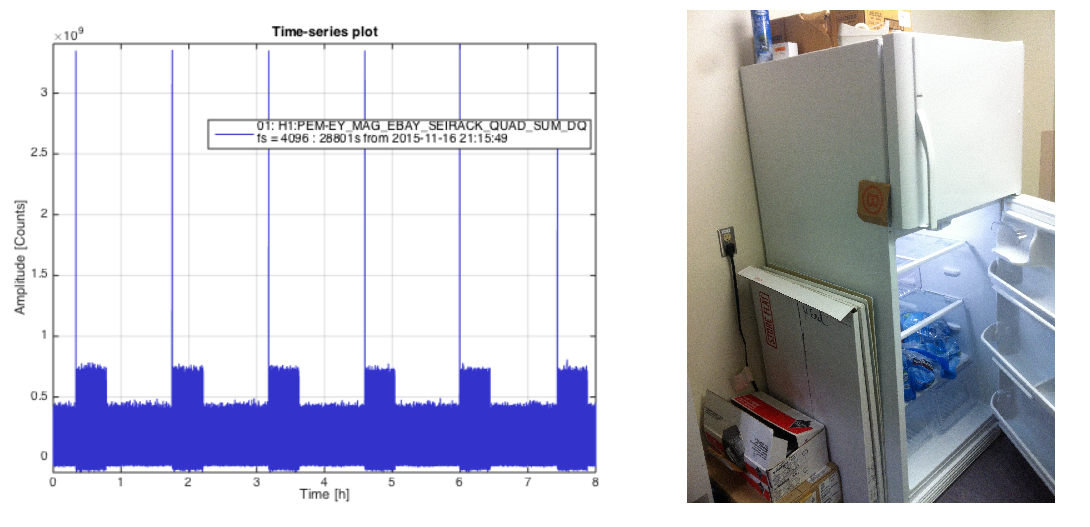
\includegraphics[width=\textwidth]{figures/fridge_plot.png}
    \caption{Left: Magnetometer plot at EY during O1 showing periodic glitches followed by temporarily elevated fields. Right: The culprit.}
    \label{fig:fridge_plot}
\end{figure*}

Periodic glitches centered around 60\,Hz occurred throughout all of O1 at LHO. Approximately once per hour a loud 60\,Hz glitch would be accompanied by increased magnetic fields at the Y end station (EY). This small magnetic field would disappear on the order of minutes and can be seen in Figure~\ref{fig:fridge_plot}. The period between glitches seemed to be slowly increasing over time. There was also a regular burst of glitches every Tuesday morning, which is maintenance day on site. These glitches appeared to be related to the use of electronics at EY, but the actual source avoided detection for many months. Magnetometers in the electronics bay showed larger spikes and post-glitch fields than the magnetometers next to the vacuum chambers, suggesting the issue was in that room. Using magnetometers plugged into oscilloscopes for portability, Borja Sorazu and I examined the entire electronics bay. The different magnetometer axes had shown different strength fields after a glitch. Rotating the magnetometers confirmed that the observed fields were real and not a rack related issue. The only piece of equipment in the room with strong magnetic fields was the Endevco\textsuperscript{\textregistered} power supply, which powers the PEM accelerometers. This was also the only device plugged into AC power via the wall. Microphones in the electronics bay had picked up a small signal when the glitches occurred, but no sound was audible to human ears.

Eventually it was noticed that glitches occurred whenever someone used the shoe cleaner, or anything else that pulled significant AC current from the wall. This would explain why there was always a burst of glitches on Tuesday mornings as workers entered the building and cleaned their shoes. Almost by chance, it was noticed that a refrigerator in the corner of the end station was plugged in. This refrigerator was surrounded by unused equipment in a makeshift storage room near the electronics bay and was not supposed to be connected to power. Unplugging the refrigerator immediately stopped the periodic 60\,Hz glitches. This also explained why the period between glitches was slowly increasing. Glitches were occurring when the compressor in the refrigerator turned on. As the weather outside got colder, the refrigerator's temperature was increasing at a slower rate, increasing the period between glitches. After this was realized, the Endevco\textsuperscript{\textregistered} power supply was further tested as a potential coupling site for these glitches. Unfortunately no good evidence was found and the exact coupling mechanism behind these glitches was never definitively proven. Regardless, the glitches have been removed from LIGO data. A summary of this work can be viewed in LHO log 23483.

\begin{figure*}[t]
    \centering
    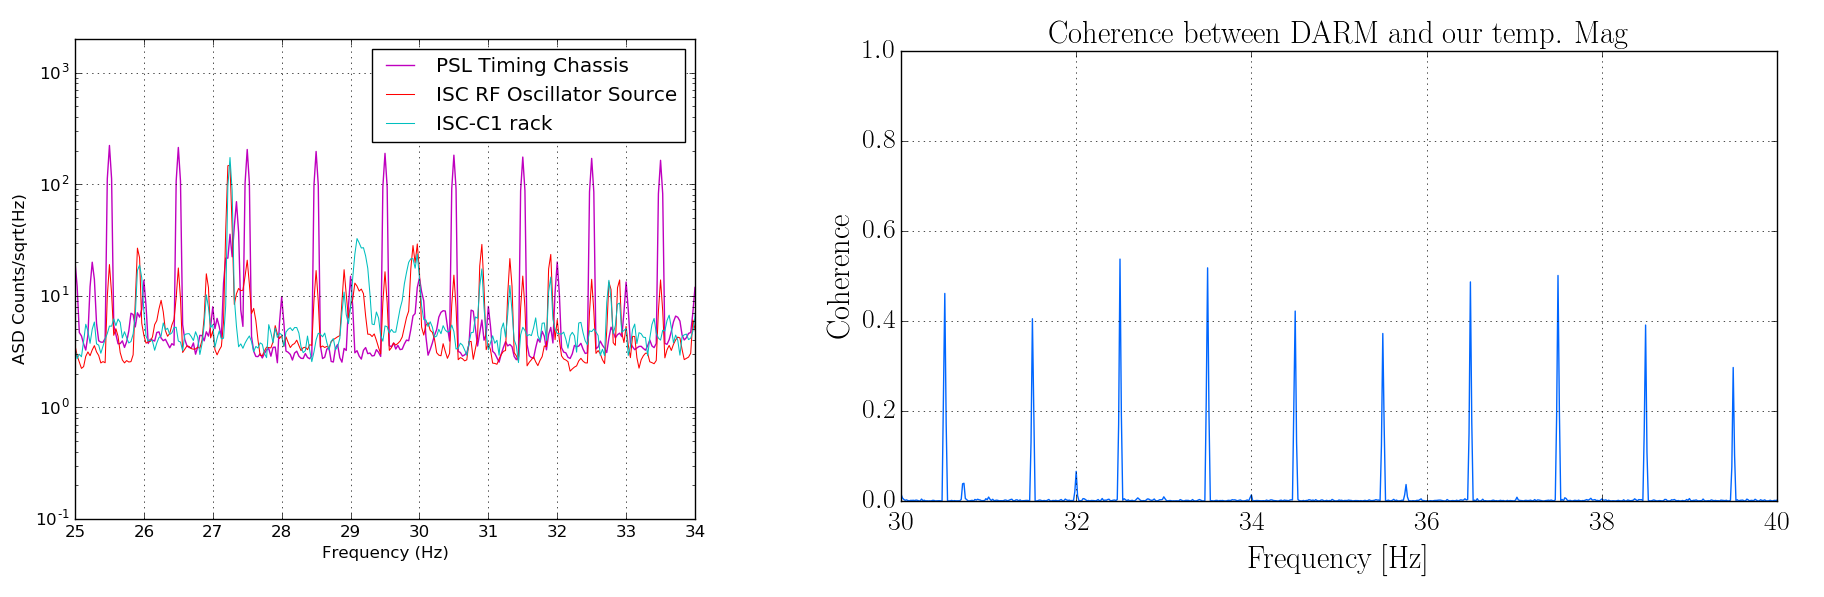
\includegraphics[width=\textwidth]{figures/LED_plots.png}
    \caption{Left: Magnetometer data from different locations at EY. Combs were strongest near timing equipment. Right: Coherence between temporary magnetometer and DARM (strain) confirming that this is the correct noise source.}
    \label{fig:LED_plots}
\end{figure*}

A strong comb with 1\,Hz spacing and 0.5\,Hz offset was also present in LIGO's data throughout O1. Several magnetometer channels at both end stations showed coherence with the strain channel. Once again portable magnetometers were used to investigate the end station with an emphasis on the electronics bay. The comb was clearly visible around nearly all electronics, but it was particularly strong around equipment associated with the timing system. Figure~\ref{fig:LED_plots} shows the combs in magnetometer data and coherence with the strain channel. The timing system contains master and slave components with LED indicators that draw power as a square wave with 2 second period. This would produce the observed comb in a Fourier series. Initially, the slave cards were placed on separate power supplies at the corner station and both end stations, however this did not reduce the strength of the comb. Replacing the power supply for the master system was considered, but ultimately it was decided to update the firmware to stop the LEDs from flashing. This did not completely remove the combs, but long term studies showed that the strength of the combs decreased by an order of magnitude. This work was published in the O1-O2 lines paper~\cite{covas2018identification}.




























